Charged particles traversing the ID leave hits along their travel path, which are used to reconstruct their trajectories. These trajectories are defined by five parameters: the transverse and longitudinal impact parameter ($d_{0}$, $z_{0}$), the azimuthal and polar angles ($\phi$, $\theta$), and the charge to momentum ratio ($q/p$) as seen in Figure~\ref{fig:track_parameters}.

\begin{figure}[hpt]
  \centering
  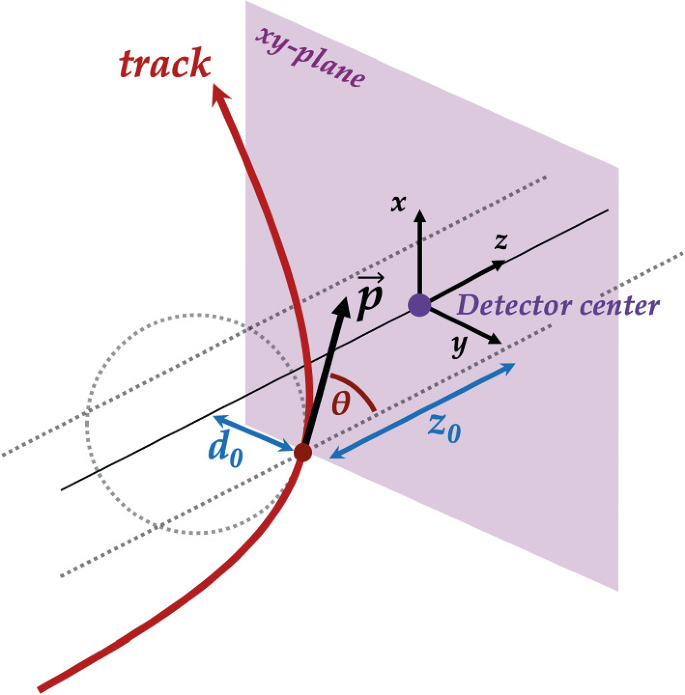
\includegraphics[width=0.55\textwidth]{figures/reco/reco_track_parameters.png}
  \caption{Illustration of the five track parameters used to define a track in the ATLAS detector. The parameters are transverse and longitudinal impact parameters ($d_{0}$, $z_{0}$), the azimuthal and polar angle ($\theta$, $\phi$), and charged divided by momentum ($q/p$). Taken from~\cite{Mironova2023}.}\label{fig:track_parameters}
\end{figure}

ATLAS track reconstruction consists of a two stages track reconstruction approach. The primary track reconstruction method for ATLAS is the inside-out algorithm which forms tracks that have $\pt > 500$ MeV with at least eight hits. It begins by identifying energy deposits in the Pixel and SCT detectors and converting them into three-dimensional space points. 

Space points in the SCT are then combined into triplets to form track seeds which represent space points that are compatible with a charged particle originating from the IP\@. In Runs 1 and 2, track seeds could be a combination of Pixel and SCT hits, however, studies in Run 3 track reconstruction, showed that these combinations resulted in high fake track rates, and therefore are no longer used.~\cite{ATL-PHYS-PUB-2023-034}.

The SCT based seeds are passed into a Kalman Filter-based track finding algorithm~\cite{kalman_filter}, which extrapolates the seeds through detector elements creating multiple track candidates. A region-of-interest (ROI) is defined along the $z$-axis using the seeds, corresponding to the luminous region of the bunch crossing. Track finding in the Pixel detector is then restricted to this ROI, discarding anything falling outside.

After candidate tracks are built, an ambiguity solving step is performed to resolve overlapping and fake tracks. A set of neural networks~\cite{ATLAS:2024vdo} are used to place limits on hit usage and track sharing to maintain low false-positive rates. Surviving track candidates undergo a global $\chi^{2}$~\cite{Cornelissen:2008zza} fit for high-precision track parameter estimation. Where possible, track candidates from the Pixel and SCT layers are extended into the TRT to improve momentum resolution and particle identification. This method reconstructs primary tracks with an isolated track efficiency of approximately 70 to 85\% depending on track $\pt$ and $\eta$. 

The primary vertex (PV) is the vertex that has the largest track $\sum \pt^{2}$ and is where the $pp$ collision took place. PV reconstruction is performed in two main steps:
\begin{description}
  \item[Gaussian Track Density Seed Finder (GS)] The GS~\cite{ATLAS:2019jmx} is used to identify vertex seeds by modeling each seed as a correlated Gaussian in the radial and longitudinal directions, centered at ($d_{0}$, $z_{0}$) and normalized to unity. A track's seed-finding density is evaluated along the $z$-axis defining a total density function that represents the sum of all nearby tracks. The maximum of this is the vertex seed location.
  \item[Adaptive Multi-Vertex Finder (AMVF)] The AMVF~\cite{cms_AMVF} is applied to the seeds to find the vertex position. It determines the compatibility between a track and seed by assigning a weight to each track. With every iteration, compatible tracks are down-weighted, and vertex position is updated. Tracks are removed and this process continues until no tracks remain.
\end{description}
Other vertices can be reconstructed are are known as the pileup vertices.
